\documentclass[14pt]{extarticle}

\usepackage[english]{babel}
\usepackage[utf8]{inputenc}
\usepackage{graphicx,eso-pic}
\usepackage{tgschola}
\usepackage{listings}
\usepackage{pdfpages}
\usepackage[nodayofweek]{datetime}
\usepackage[bottom=2.25cm,top=3.75cm,left=1.5cm,right=1.5cm]{geometry}
\usepackage{xcolor}

\fontfamily{qcs}
\pagenumbering{gobble}

\lstdefinestyle{mystyle}{
    basicstyle=\normalsize,       
    breaklines=true,                                 
    keepspaces=true,                                    
    numbersep=5pt,                  
    showspaces=false,                
    showstringspaces=false,
    showtabs=false,                  
    tabsize=2
}

\lstset{style=mystyle}

% Add header and footer images
\AddToShipoutPictureBG{%
  \AtPageUpperLeft{%
    \raisebox{-\height}{%
    
\includegraphics[width=\paperwidth]{private/header.jpeg}}
  }
  \AtPageLowerLeft{%
    \makebox{%
    
\includegraphics[width=\paperwidth]{private/footer.jpeg}}
  }
}

% Set title
\title{%
    \textbf{
    \vspace{-3em} \\ 
    \Large Experiment Number \\
    \vspace{-4em}
    }
}

% Remove author and Date
\author{}
\date{}

\begin{document}

\maketitle % Add title of doc

% Add the name and details
\section*{}
    \begin{tabular}{ llp{2cm}ll } 
        Name :: & Rishabh Anand & & UID :: & 19BCS4525  \\ 
        Branch :: & CSE - IoT & & Sec/Grp :: & 1/A \\ 
        Semester :: & 5\textsuperscript{th} & & Date :: & \shortdate{\today} \\
        % Subject :: & Adv Programming Lab & & CODE :: & CSP-347  \\ 
        % Subject :: & Embedded System Lab & & CODE :: & CSD-333  \\ 
        % Subject :: & DIOT Lab & & CODE :: & CSD-337  \\ 
        Subject :: & WSN Lab & & CODE :: & CSD-331  \\ 
    \end{tabular}
    
\vspace{1em}

\section*{\normalsize 1. Aim :}

\section*{\normalsize 2. Task :}

\begin{itemize}
  \item 
\end{itemize}

\section*{\normalsize 3. Requirements :}

\begin{enumerate}
  \item Arduino Board
  \item RGB LED
  \item Potentiometer
  \item Power Source
  \item Connecting Wires
  \item BreadBoard
  \item Resistors (230 ohm)
\end{enumerate}

% \section*{\normalsize 3. Algorithm :}

%    \begin{enumerate}
%     \item 
%    \end{enumerate}

% Auto add code and output
\newpage
\section*{\normalsize 4a. Steps / Source Code :}

\begin{enumerate}
  \item Connect three wires to the Arduino board. 
  \item The first goes to ground from one of the outer pins of the potentiometer. 
  \item The second goes from 5 volts to the other outer pin of the potentiometer. 
  \item The third goes from analog input 2 to the middle pin of the potentiometer.
\end{enumerate}

\lstinputlisting{temp/code.cpp} 

\section*{\normalsize 5a. Observations :}

\begin{center}
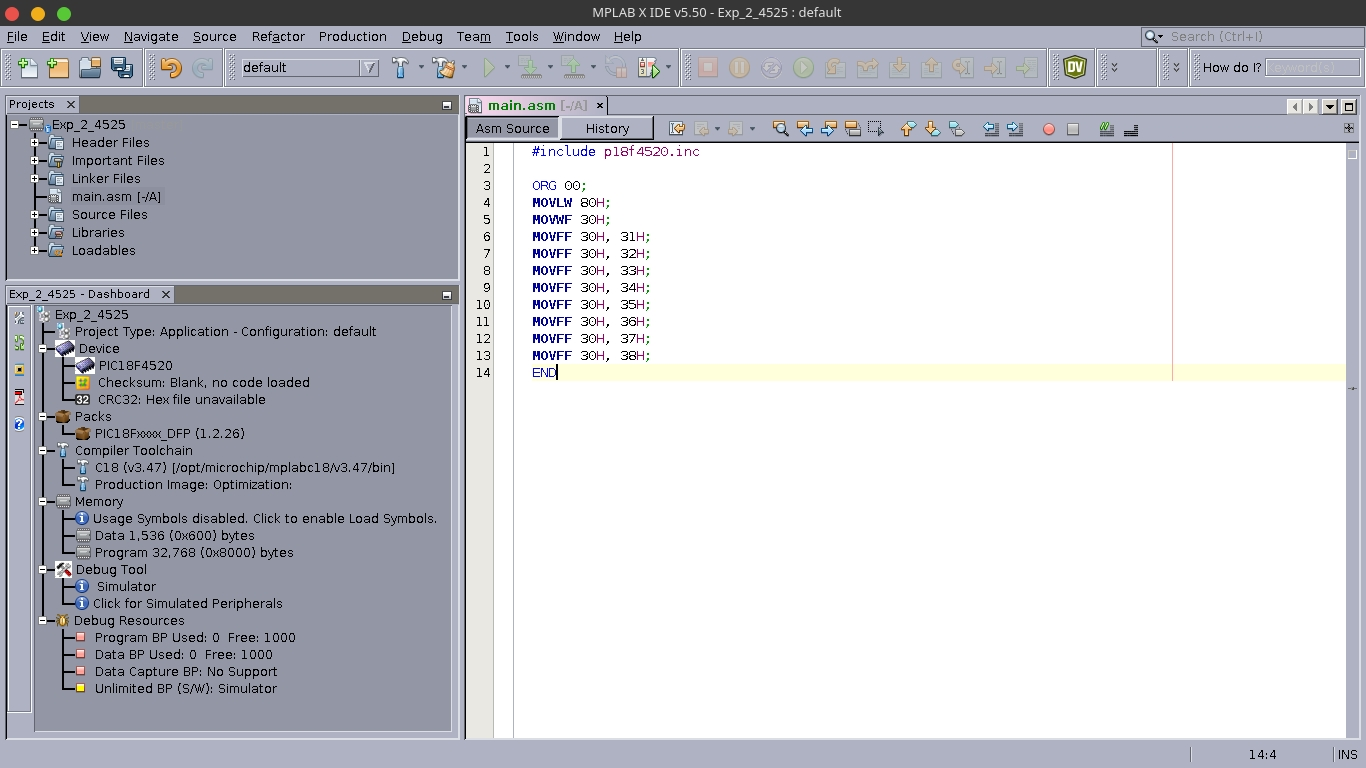
\includegraphics[scale=0.5]{temp/1.jpeg}\\

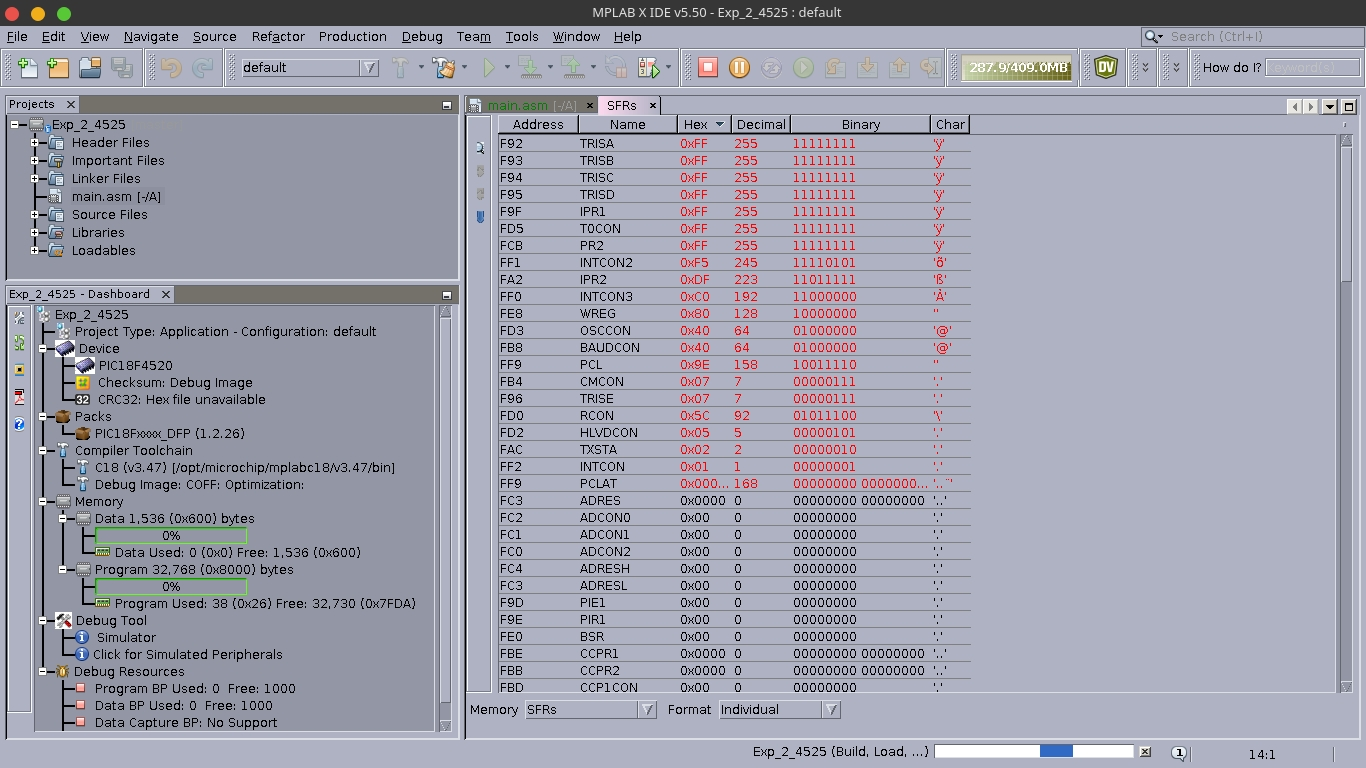
\includegraphics[scale=0.5]{temp/2.jpeg}\\

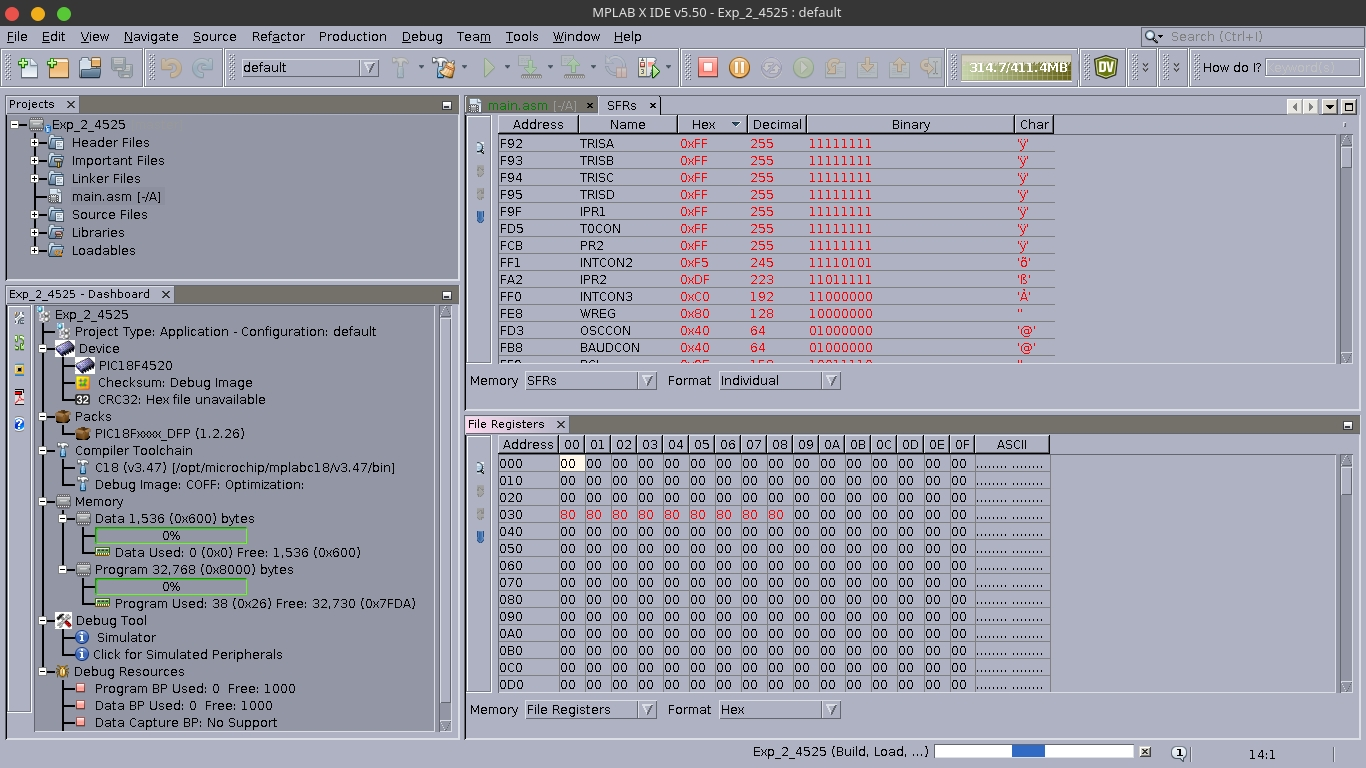
\includegraphics[scale=0.5]{temp/3.jpeg}
\end{center}

\newpage
\includepdf[pages={2,3,4}]{temp/Exp2.pdf}
\section*{\normalsize Learning Outcomes :}
  
  \begin{itemize}
    \item Arduino Uno
    \item LED Working
    \item Arduino IDE
    \item Potentiometer Working
    \item Resistors Working
  \end{itemize}

\section*{}

\begin{center}

\begin{tabular}{ |p{2.5cm}|p{4cm}|p{5cm}|p{5cm}|} 
 \hline
 S. No. & Parameters & Marks Obtained & Maximum Marks \\
 \hline
 1.&&&\\
 \hline
 2.&&&\\
 \hline
 3.&&&\\
 \hline
 &&&\\
 &&&\\
 \hline
\end{tabular}
\end{center}

\end{document}
